\documentclass[a4paper,10pt]{article}

\usepackage{subfig}
\usepackage{float}
\usepackage{graphicx}

%opening
\title{Degree-dependent Social Network Models}
\author{Sam Magura, Vitchyr Pong}

\begin{document}

\maketitle

\section{Introduction}

%Here we present two similar dynamic network processes that exhibit drastically different macroscopic behavior. In an iteration, we choose a node $v_0$ and break one of its incident edges.. Then, for a node $v'$ that is not adjacent to $v_0$ we add a new edge $\{v_0, v'\}$. This behavior reflects real social behavior; relationships with popular, well-connected people are potentially more valuble than relationships with less well-connected people. The model takes a parameter $I$ --- a measure of \emph{intolerance} toward unpopular people --- that determines the extent to which the degrees of adjacent nodes affect the breaking probabilities. We predicted that changing $I$ would make the model behave differently, but our simulations showed no relationship between $I$ and the model's macroscopic behavior.

\section{Model Definition}

The process operates on a graph $G = (V, E)$.

\paragraph{Definitions}
\begin{itemize}
 \item A vertex $v \in V$ is a member of the set $\mathbf{V_1}$ if and only if $0 < deg(v) < |V| - 1$.
 \item A vertex $v \in V$ is a member of the set $\mathbf{V_{out}(v_0)}$ if and only if $v \neq v_0$ and $\{v, v_0\} \notin E$. 
\end{itemize}

\paragraph{Outline} An iteration consists of the following steps. The specifics of the breaking choice and the rewiring choice are defined separately for each of the two models.

\begin{enumerate}
 \item Choose a vertex $v_0$ randomly from $V_1$. 
 \item \emph{The breaking choice.} Choose an edge $\{v_0, v^*\} \in E$. 
 \item \emph{The rewiring choice.} Choose a vertex $v' \in V_{out}(v_0)$.
 \item Remove the edge $\{v_0, v^*\}$ from the graph.
 \item Add an edge $\{v_0, v'\}$ to the graph.

\end{enumerate}

Performing these steps will always be possible, provided $|V_1| > 0$. Otherwise, a $v_0$ could not be selected. Because $v_0$ is in $V_1$, it has at least one incident edge. This edge may be chosen in the breaking choice and broken. On other hand, because $v_0$ is in $V_1$, there also exists at least one vertex $v' \in V$ that $v_0$ is not adjacent to. This vertex may be chosen in the rewiring choice. 

\subsection{Breaking-function Model}

Define the behavior of the \emph{breaking-function model} as follows.

\begin{description}
 \item[The breaking choice]

 Let the chance that some edge $\{v_0, v\} \in E$ is chosen be proportional to

 \begin{equation}
\label{eqn:breaking-function}
 B(v) = \frac{I}{deg(v)} + \frac{1 - I}{\overline{deg}}
 \end{equation}

where $\overline{deg}$ is the mean degree of the vertices in the graph. $I$ is in the range $[0, 1]$. This is the \emph{breaking function}. We chose to use the mean degree here because the values of the two terms of the breaking function should be balanced. Additionally, the second term should be independent of $v_0$ and $v$.

 \item[The rewiring choice] Randomly select a $v'$ from $V_{out}(v_0)$.
\end{description}

\subsection{Rewiring-function Model}

Define the behavior of the \emph{rewiring-function model} as follows.

\begin{description}
 \item[The breaking choice] Let each edge incident on $v_0$ have the same chance of being broken.

 \item[The rewiring choice] For a vertex $v \in V_{out}(v_0)$, let the chance that $v$ is selected be proportional to

 \begin{equation}
\label{eqn:rewiring-function}
 R(v) = I \cdot deg(v) + (1 - I) \cdot \overline{deg}
 \end{equation}

where $\overline{deg}$ is the mean degree of the vertices in the graph. This is the \emph{rewiring function}. Unlike in the breaking function, $I$ is in the range $[0, 1)$. We do not allow $I$ to equal 1 in order to avoid a potential problem. If $I = 1$, and each vertex in $v \in V_{out}(v_0)$ has a degree of 0, then $R(v) = 0$ for each $v$, and the rewiring choice cannot be made. 
  
\paragraph{} The mean degree is used in the rewiring function because the values of the two terms should be balanced. Additionally, the second term should be independent of $v_0$ and $v^*$.

\end{description}

\section{Empirical Results}

We implemented the two variations of the model in the Python programming language. In our implementation, the initial graph is $G(n, M)$ Erdos-Renyi random graph. We wrote an additional script to run the model many times with different values of $I$ to see if the behavior of the model depended on $I$ in a significant way. For each trial, the script !!!!!!!!It then gathered several statistics on the resultant graph: number of nodes in largest component, diameter of largest component, and number of components. We predicted that the size and diameter of the largest component would increase with $I$, while the number of components would decrease with $I$. 

\subsection{Breaking-function Model}

\begin{figure}[H]
\begin{center}
\subfloat{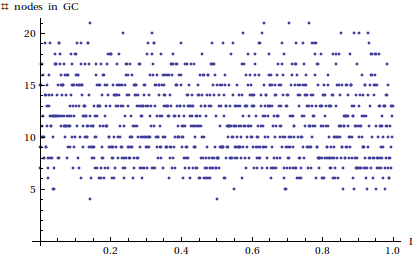
\includegraphics[height=4cm]{images/gc_size.png}}
\subfloat{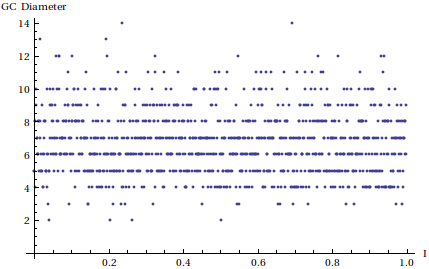
\includegraphics[height=4cm]{images/gc_diameter.png}}
\caption{Size and diameter of the largest component, for 40 nodes, 20 edges, and 1000 iterations per trial.}
\end{center}
\end{figure} 

\begin{figure}[H]
\begin{center}
\subfloat{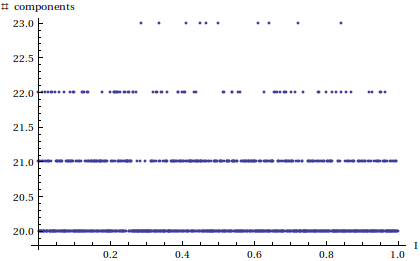
\includegraphics[height=4cm]{images/n_components.png}}
\subfloat{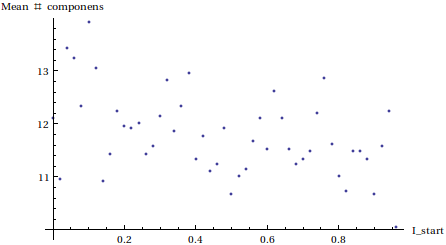
\includegraphics[height=4cm]{images/n_components_mean.png}}
\caption{Number of components and 20-trial means for number of components --- using 40 nodes, 20 edges, and 1000 iterations per trial.}
\end{center}
\end{figure} 

%We did not notice a substantial correlation between $I$ and the size of largest component, the diameter of the largest component, or the number of components. There appears to be a very slight negative correlation between $I$ and the 20-trial number-of-component means.

%In order to see why there were no correlations, we tracked the size and diameter of the largest component of the graph as iterations were performed. The following plot of size of largest component versus iteration number $i$ explains why there were no correlations. 

\begin{figure}[H]
\label{fig:gc-size-iter}
\begin{center}
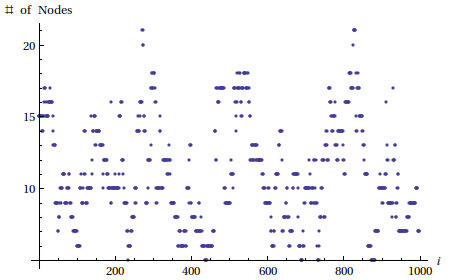
\includegraphics[height=5cm]{images/gc_size_iter.png}
\caption{How the size of the largest component changes as iterations are performed. The plot for diameter of largest component was similar.}
\end{center}
\end{figure} 
The plot shows that the model is not stable, i.e. the size of the largest component does not approach a specific value. This is to be expected because an edge is broken each iteration, no matter what. The previous plot shows that, often times, over half of the graph's 20 edges are in the largest component. In an iteration where one of these edges is brokeng, the size of the largest component can only decrease or remain the same. Additionally, the value of $I$ does not restrict the graph from reaching any given state; at most, the value of $I$ could make a certain state less likely to reach. With the size of the largest component ranging from 5 to 21 --- for a graph with 40 nodes and 20 edges --- the existence of a correlation between this property of the graph and $I$ seems unlikely.

\subsection{Model Variations}
In attempt to get more interesting results, we tried several changes to the model. None of the changes produced correlations between $I$ and any of the three quantities we recorded.

\begin{itemize}

 \item We tried to change the probability function to increase the effect of $I$ on the breaking probabilities. For example,
 \begin{equation}
  \frac{I^2}{deg(v^*)} + \frac{(1 - I)^2}{deg(v_0)}
 \end{equation}
and
 \begin{equation}
  \frac{sin(\frac{\pi}{4}I)}{deg(v^*)} + \frac{cos(\frac{\pi}{4}I)}{deg(v_0)}.
 \end{equation}

 \item Instead of using a probability function, we modified the model so that $v_0$ would always break its connection with its neighbor of least degree --- and if there were multiple neighbors of least degree, chose which one to break with randomly. 

\end{itemize}
 None of these changes produced correlations.


\end{document}
